\section{Project Management}\label{sec:projectmanagement}
According to Section~\ref{subsec:sdp} we are using Software Development Life Cycle (SDLC) as our software development process. There are various method of SDLC. Among them we are using Agile SDLC method. Also, there are various Agile methodologies. Here we are using Scrum methodology. This can be shown as follows.

\begin{figure}[H]
    \centering
    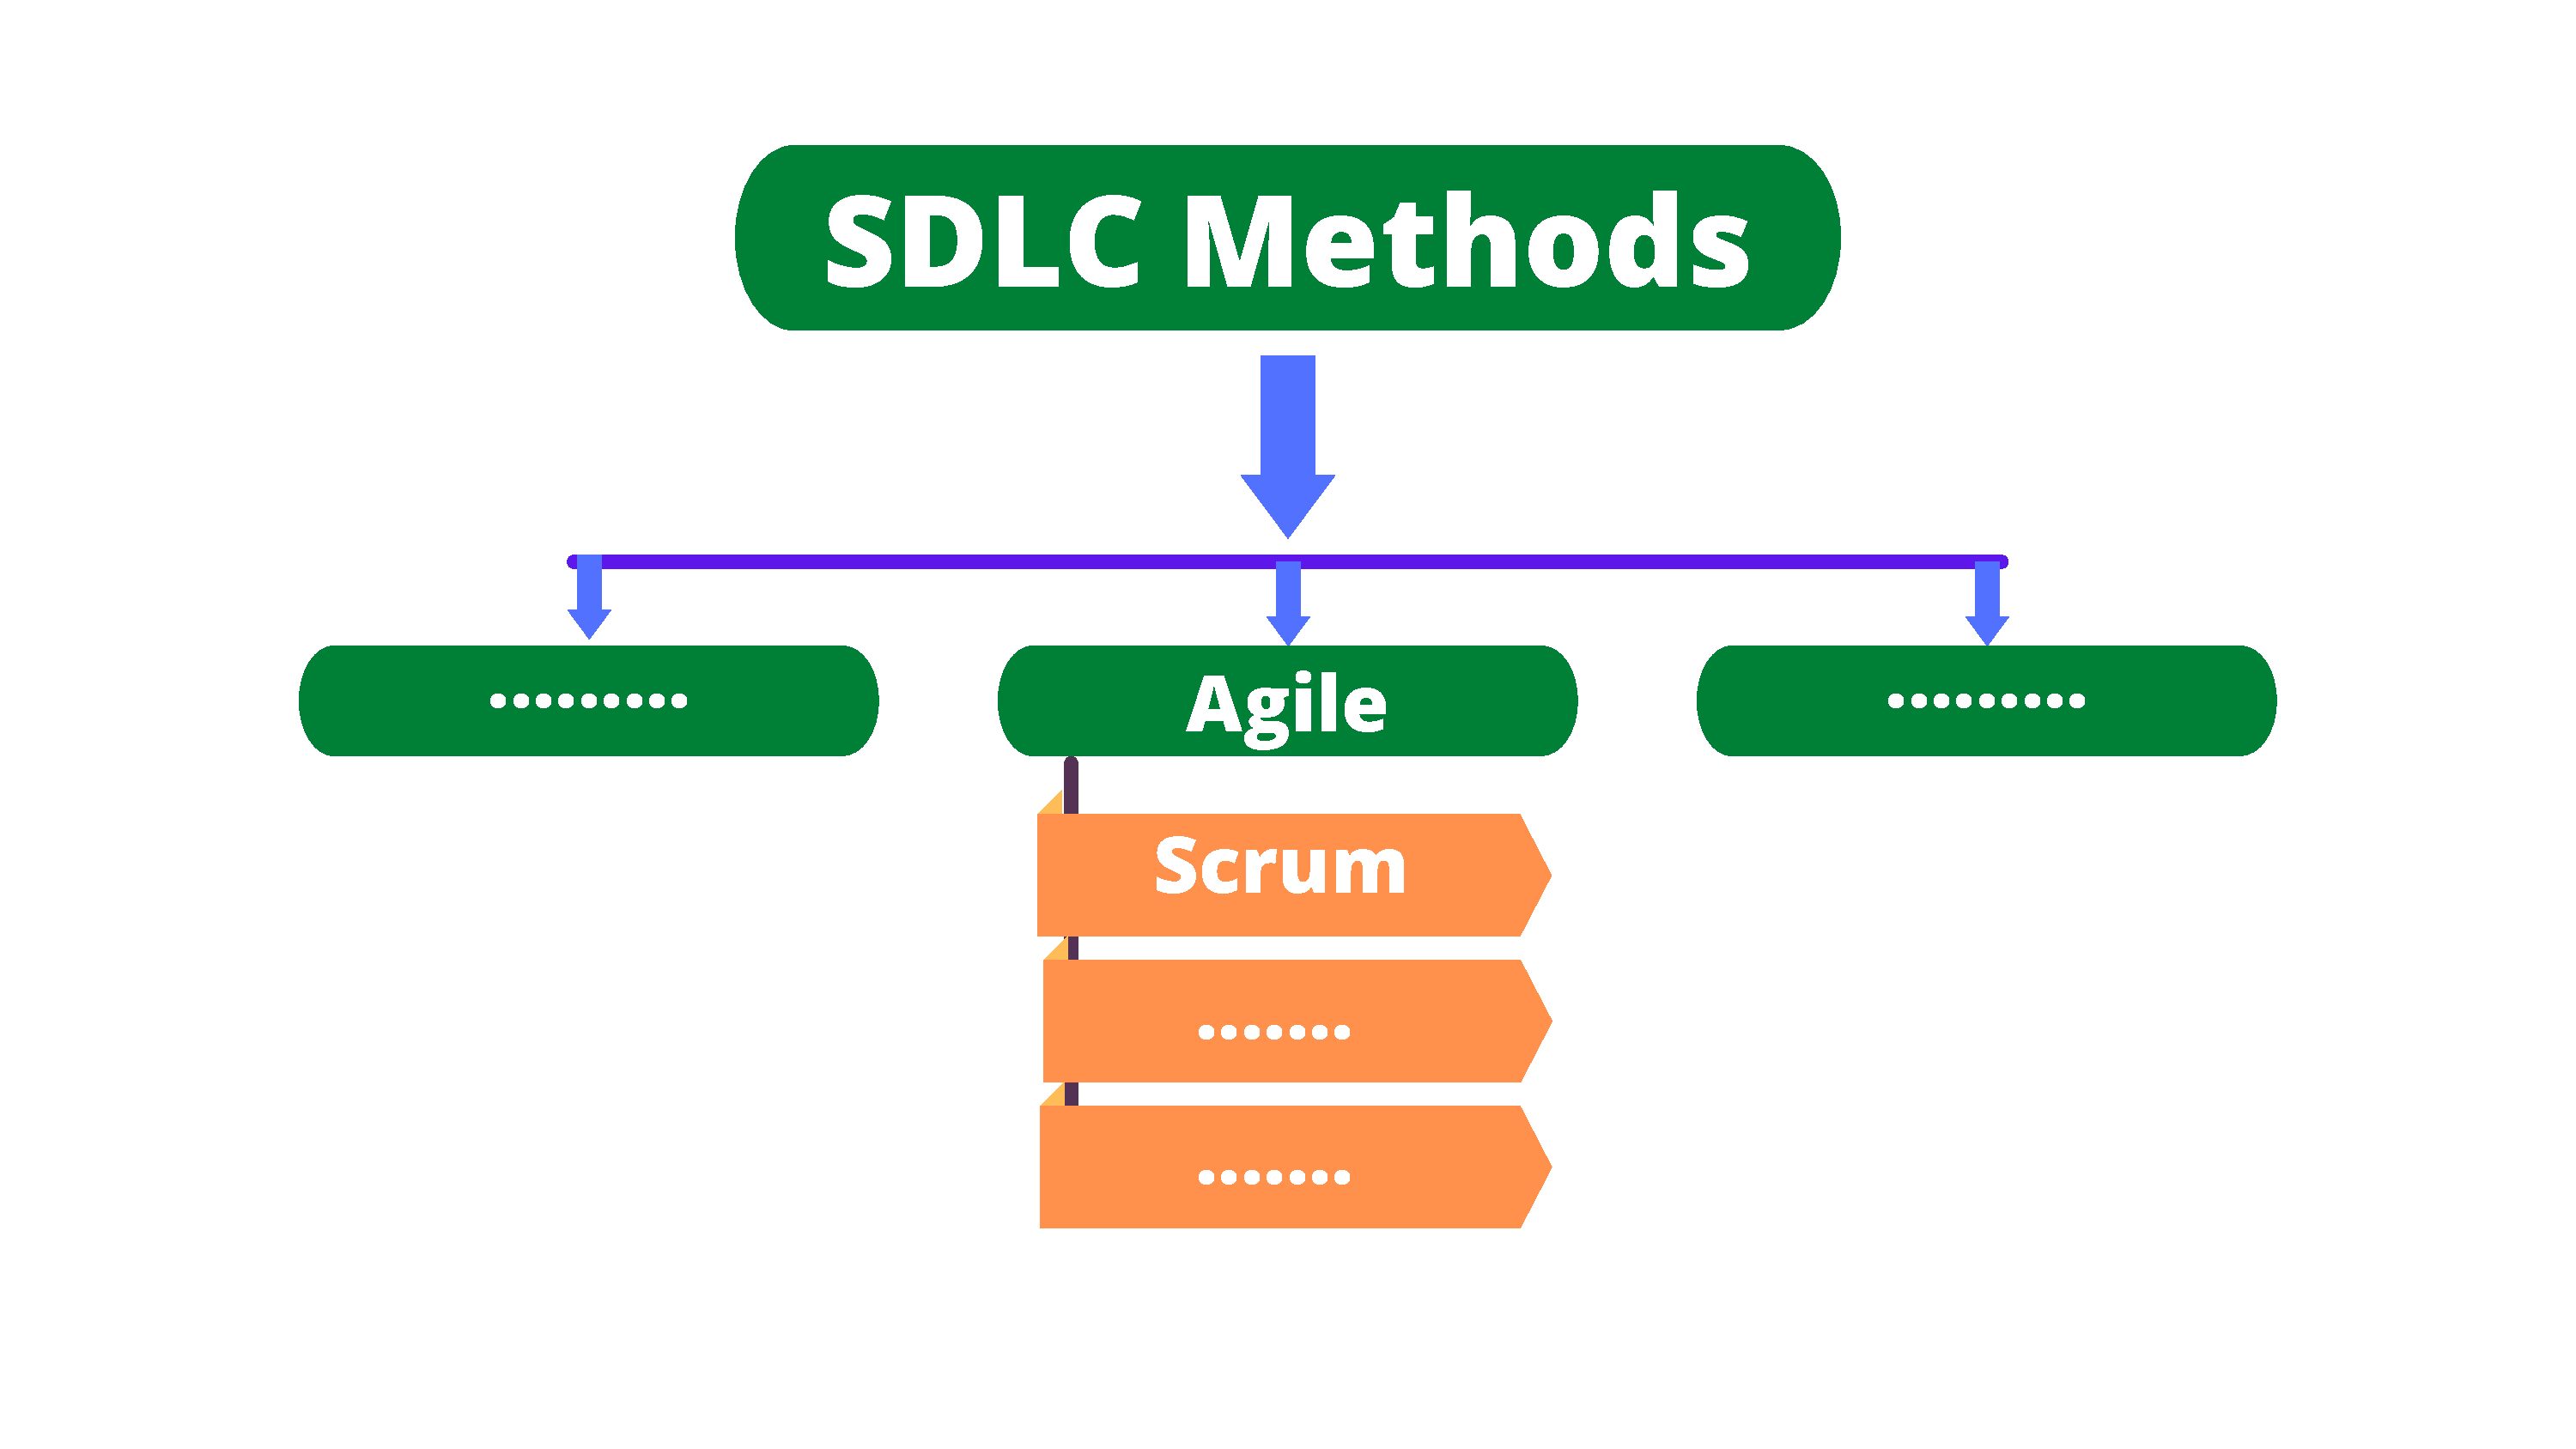
\includegraphics[width=1\textwidth]{images/SDLCMethods}
    \caption{SDLC classification}
    \label{fig:sdlc-class}
\end{figure}

The Agile SDLC model is a combination of iterative and incremental process models with a focus on process adaptability and customer satisfaction by rapid delivery of working software products. Agile Methods break the product into small incremental builds. These builds are provided in iterations. Each iteration typically lasts from about one to three weeks.
Every iteration involves cross-functional teams working simultaneously on various areas like −
\begin{itemize}
\item Planning/Requirement Gathering
\item Requirements Analysis
\item Database Modeling
\item Architectural Design
\item Implementation
\item Testing and Validation
\end{itemize}

Ref: [www.tutorialspoint.com/sdlc/sdlc\_agile\_model.htm]
Agile model believes that every project needs to be handled differently and the existing methods need to be tailored to best suit the project requirements. In Agile, the tasks are divided to time boxes (small time frames) to deliver specific features for a release.\\

Iterative approach is taken and working software build is delivered after each iteration. Each build is incremental in terms of features; the final build holds all the features required by the customer.


Here is a graphical illustration of the Agile Model −
\begin{figure}[H]
    \centering
    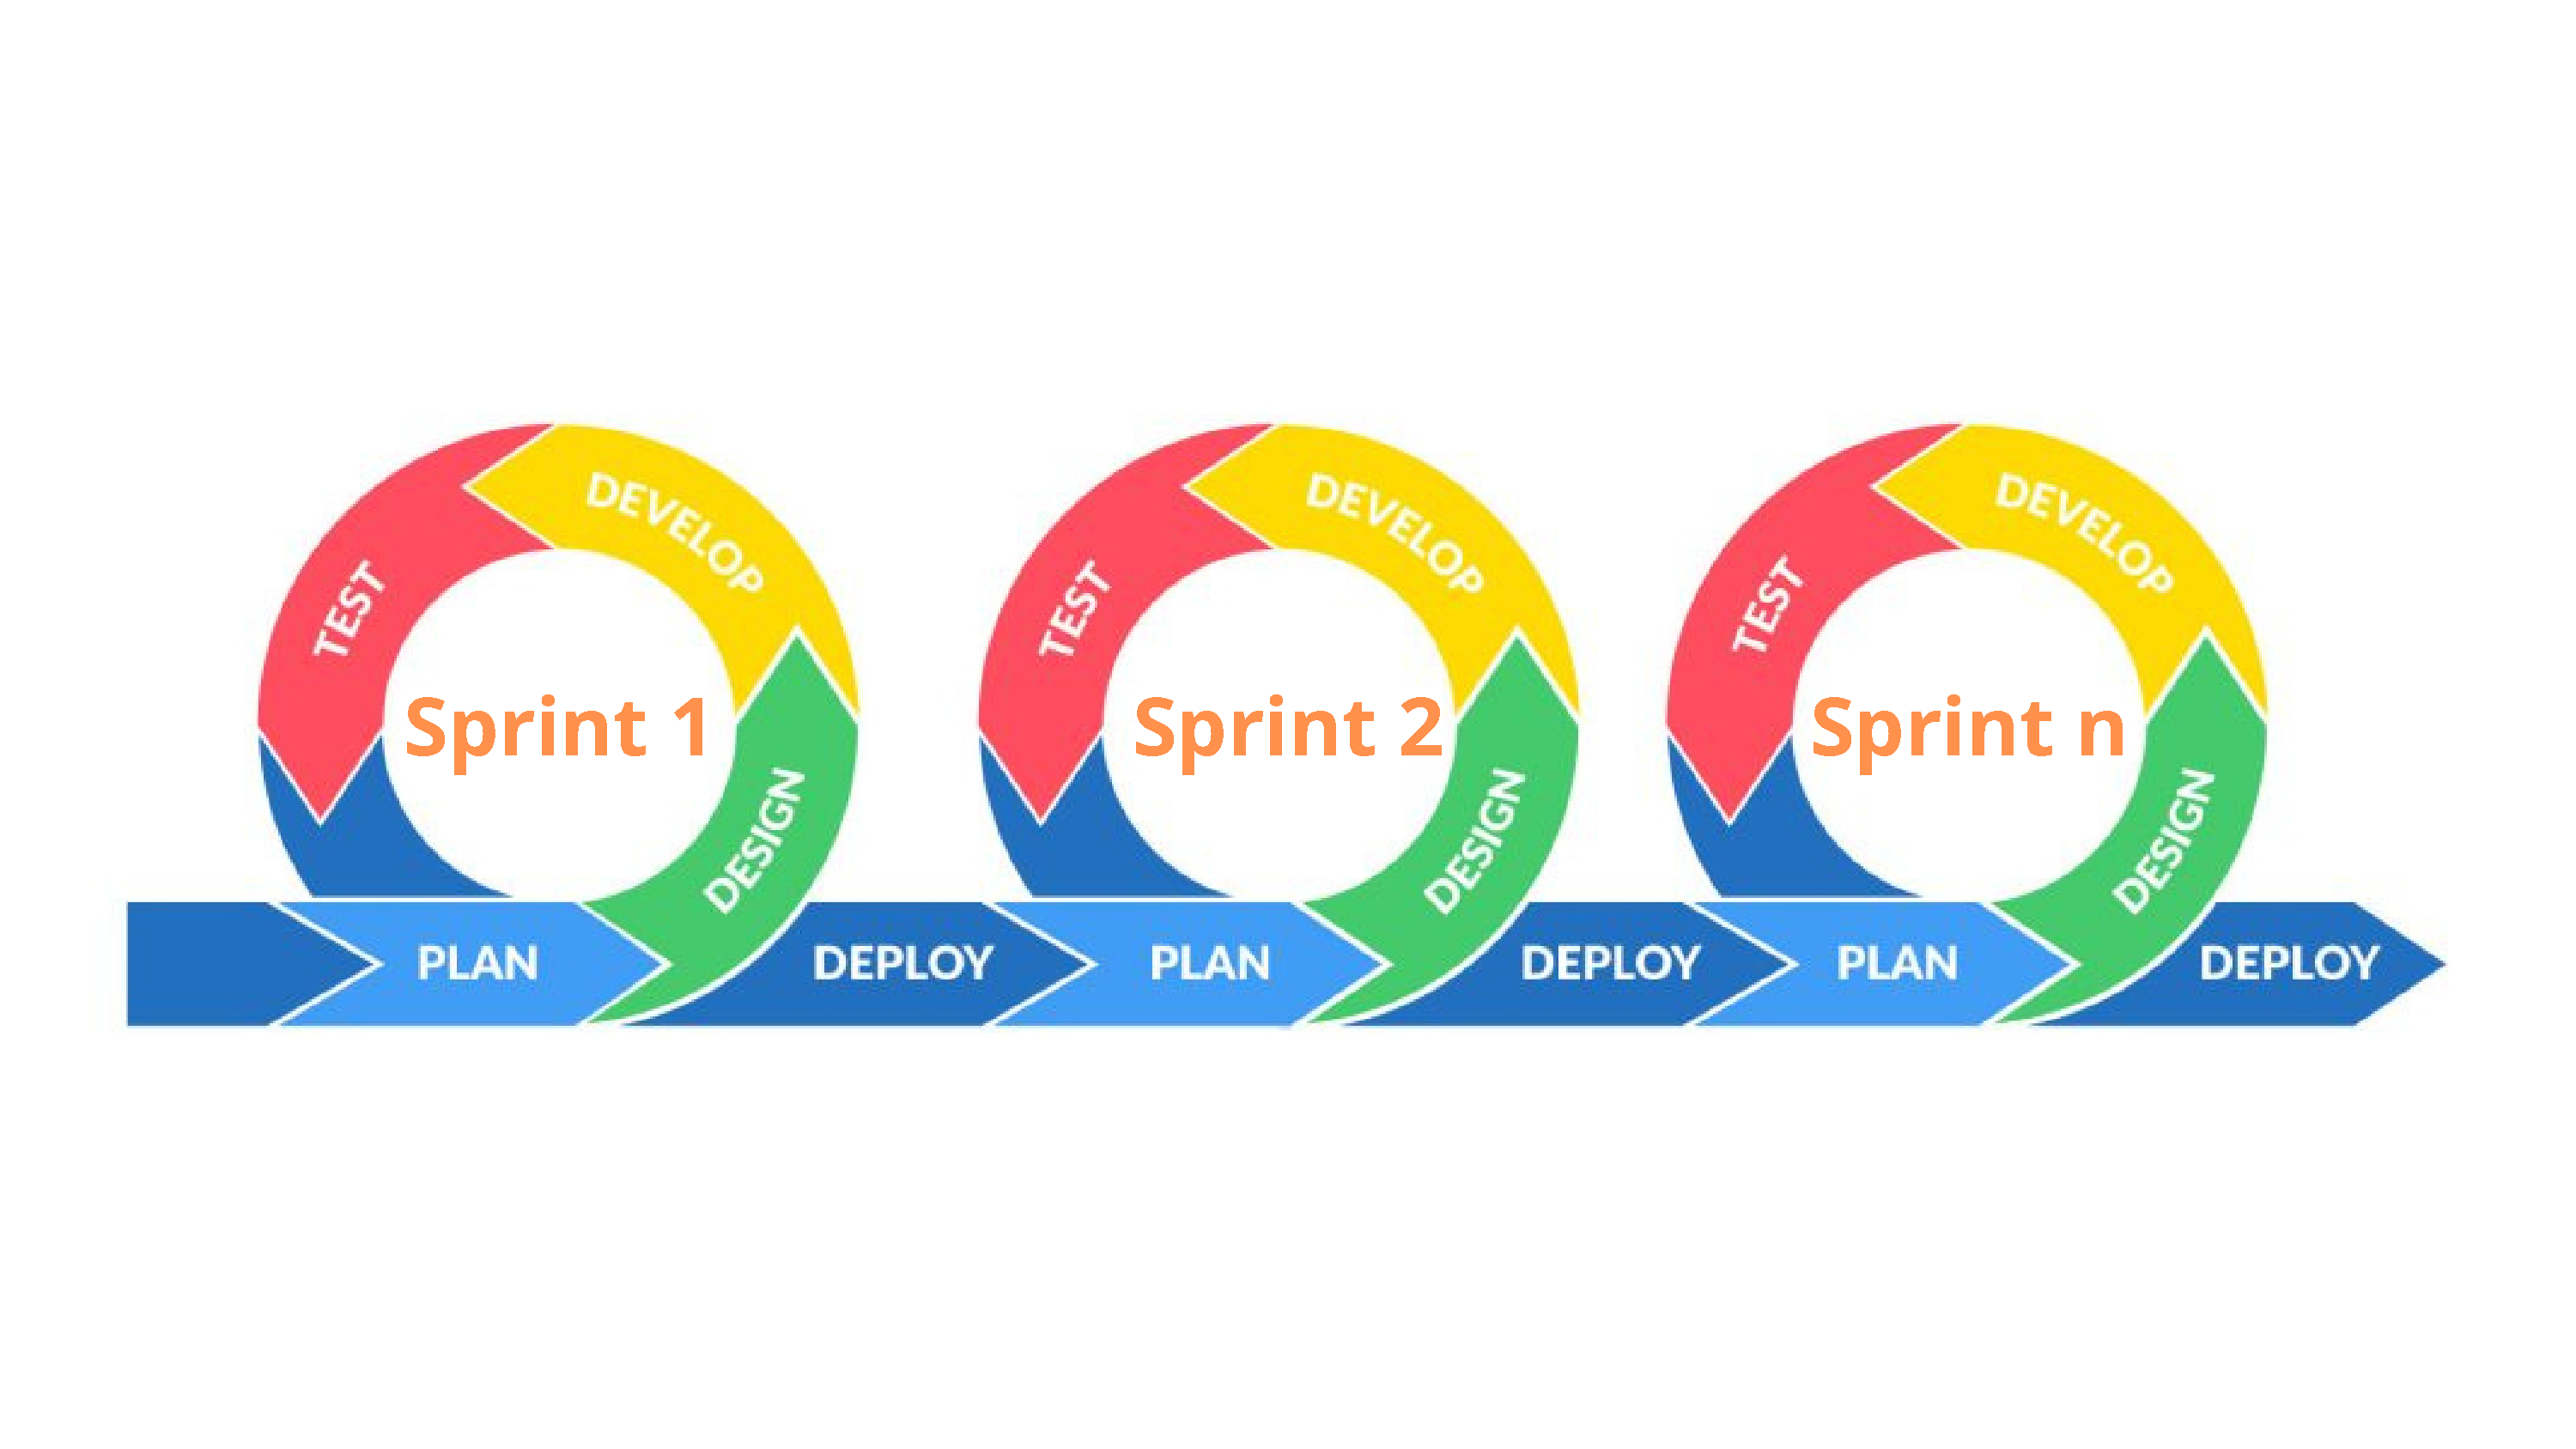
\includegraphics[width=1\textwidth]{images/agile}
    \caption{Agile Model}
    \label{fig:agile}
\end{figure}
We define separate phases (sprints in Scrum terminology) for each and every steps of SDLC. For each phase we make a plan, design a work-flow, develop it, and finally test the output of the phase. If the output is correct according to the requirements, then we proceed for the next phase.\\

To complete each of these phases or sprints we followed the Scrum methodology. It actually allows implementing Agile development methodology. So it can be called a framework which enables an iterative and incremental development process. At the end of each step a usable product is delivered to a customer. Customer feedback helps reveal possible problems or change the initial development plan if needed.\\
Here are the main roles involved in the development process, according to the Scrum model:
\begin{description}
\item[Product owner :] The product owner takes care of the end user’s interests. In our project \textit{Tonmoy Chandro Das} plays this role of a product owner. 

\item[Scrum master :] The Scrum master coordinates the whole development process. Another task is to make sure that Scrum is used properly and to hold regular Scrum meetings. In our case, \textit{Md Masud Majumdar} plys the role of team leader from the beginning to the conclusion, and he planned and executed the whole project.

\item[Scrum team :] The Scrum team develops the product. Its main tasks are programming, analysis, testing, etc. Our scrum team contains all of the members of our database team including-
\begin{itemize}
\item Md. Masud Mazumder
\item Tonmoy Chandro Das
\item Palash Hossen
\item Tareq Rahman Likhon Khan
\item Hamza Mohtadee Ibne Mamun
\item Nu Sai Mong Marma
\end{itemize}

Each scrum team member has significant contributions to various aspects of the overall project. For example we holds regular virtual meetings where all the teammates together discuses, came up with all the various ideas to design the database schema etc. The meetings we hold virtually through Google Meet and Zoom software (Online software for meetings) conducts \textit{Tareq Rahman Khan}. Within a week, we decided to draw the first E-R Diagram on our ideas which was fianlly done by \textit{Palash Hossen}. Later it was modified by \textit{Nu Sai Mong Marma}.\\

%While developing the system, we used Github (an online code library used to version control mainly) to make the collaboration among teammates and to integrate all the assigned task and make the final system. Github not only allows us to collaborate with our teammates but also to control the modifications of the application. Since the start of the project, our team made about 100 of commits into Github repository. All the commits are from \textit{Tonmoy Chandro Das} and \textit{Md. Masud Majumdar} as frontend and backend funcionalities were developed by them. To interact with github, we used git in our local machine and Visual Studio Code as code editor.\\%

While developing the system, we also looked after the documentation of this entire project. This documentation was prepared under the leadership of \textit{Hamza Mohtadee Nafi}.\\

\textit{Md. Masud Mazumder} and \textit{Tonmoy Chandro Das} write codes to implement our system mostly.

\end{description}

Now, let’s take a look at the main steps of the development process that Scrum consists of which we followed.

\begin{enumerate}
\item \textbf{Product Backlog Creation}\\
In this process, we transformed the significance and functional details of the system into short stories. Every user story gets a unique ID. As a rule, user stories have the following format: As a [User Role], I want to [feature body] so that [User profit]. This list below shows how these stories can look like. These are actual product requirements that were implemented during the software developing process:
\begin{table}[h]
\centering
\huge
\resizebox{\textwidth}{!}{
\begin{tabular}{|l|l|l|}
\hline
UserID & User Type & User Story \\ \hline
user-01 & Student & I want to pay all my tuition fees via online from anywhere in the world. \\ \hline
user-02 & Student & I want to see all of my previous transactions and due transactions that I need to complete. \\ \hline
user-003 & Administrative personnel & I need to create, update and edit payments for each and every students. \\ \hline
user-04 & Administrative personnel & I want to have track of the payments for all the students. \\ \hline
user-05 & Teacher & I need to collect attendance online for each and every classes I take. \\ \hline
\end{tabular}
}
\caption{\label{tab:userStory}User story example.}
\end{table}

After listing all the product backlog items, it's time to sort through them and prioritize the tasks that which tasks are more important than others. Most important one is ranked higher than less important one. This is called prioritization. We then make a list ordering according to the priority in descending order. This one is a continuous process. Because we continuously add a new item in the backlog list and prioritize it and update the listing.



%As an example, consider a standard student whose semester final test is scheduled for a few days from now. He/she will be required to pay the semester fee within a certain time frame determined by the administration. Students suffer as a result of this, and their preparedness is negatively impacted. Furthermore, while using the traditional method of transaction, a university is completely reliant on a single bank branch, which creates a tiring and agonizing scenario when a large number of students seek to pay their tuition fees on the same day as the university. Several students even fail to submit their fees on time since they are unable to conduct any financial activities during non-working hours. Teachers are also said to have lost around one-third of the course session while manually collecting attendance, which has an adverse impact on the focus of pupils. On the other aspect, management often complains about how time-consuming it is to manually update student data in papers. It not only takes a long time to finish, but it also needs the actual presence of a huge number of individuals in order to be successful. These considerations inspired our team's decision to design a single application using the information obtained from our database course that is capable of resolving all of the challenges discussed above.%

\item \textbf{Sprint planning and creating backlog}\\

Second step of Scrum methodology is sprint planning and creating sprint backlog. One of the most important task of this step is to make a duration of each sprint. As there is a time frame for the respective ``Database Systems" course, we have determined our sprint duration for about 1 to 2 weeks. We have set a goal for each and every sprint.\\
After that we our product owner determines importance of user story and Scrum team selects the most important user stories from the product backlog. Thus the sprint backlog is created which will be completed during the respective sprint.

\item \textbf{Working on sprint}\\

This is a phase of practical application. The real stories is reorganized as a discrete task in the sprint backlog, which is where the actual work begins. In order to get started, we create a task board, also known as a Scrum board with a large number of cards in use. A scrum board is mainly a collection of tasks of a sprint. Each task is represented by a single card in a scrum board. The cards can be arranged according to their importance. When work on a task has been started, the corresponding card is moved from the “To do” field to the “In progress” one. When work is completed, the card is moved to the “Testing” field, and after the task is successfully tested, the card goes to the “Done” field. An example of a Scrum board is shown below.

\begin{figure}[H]
    \centering
    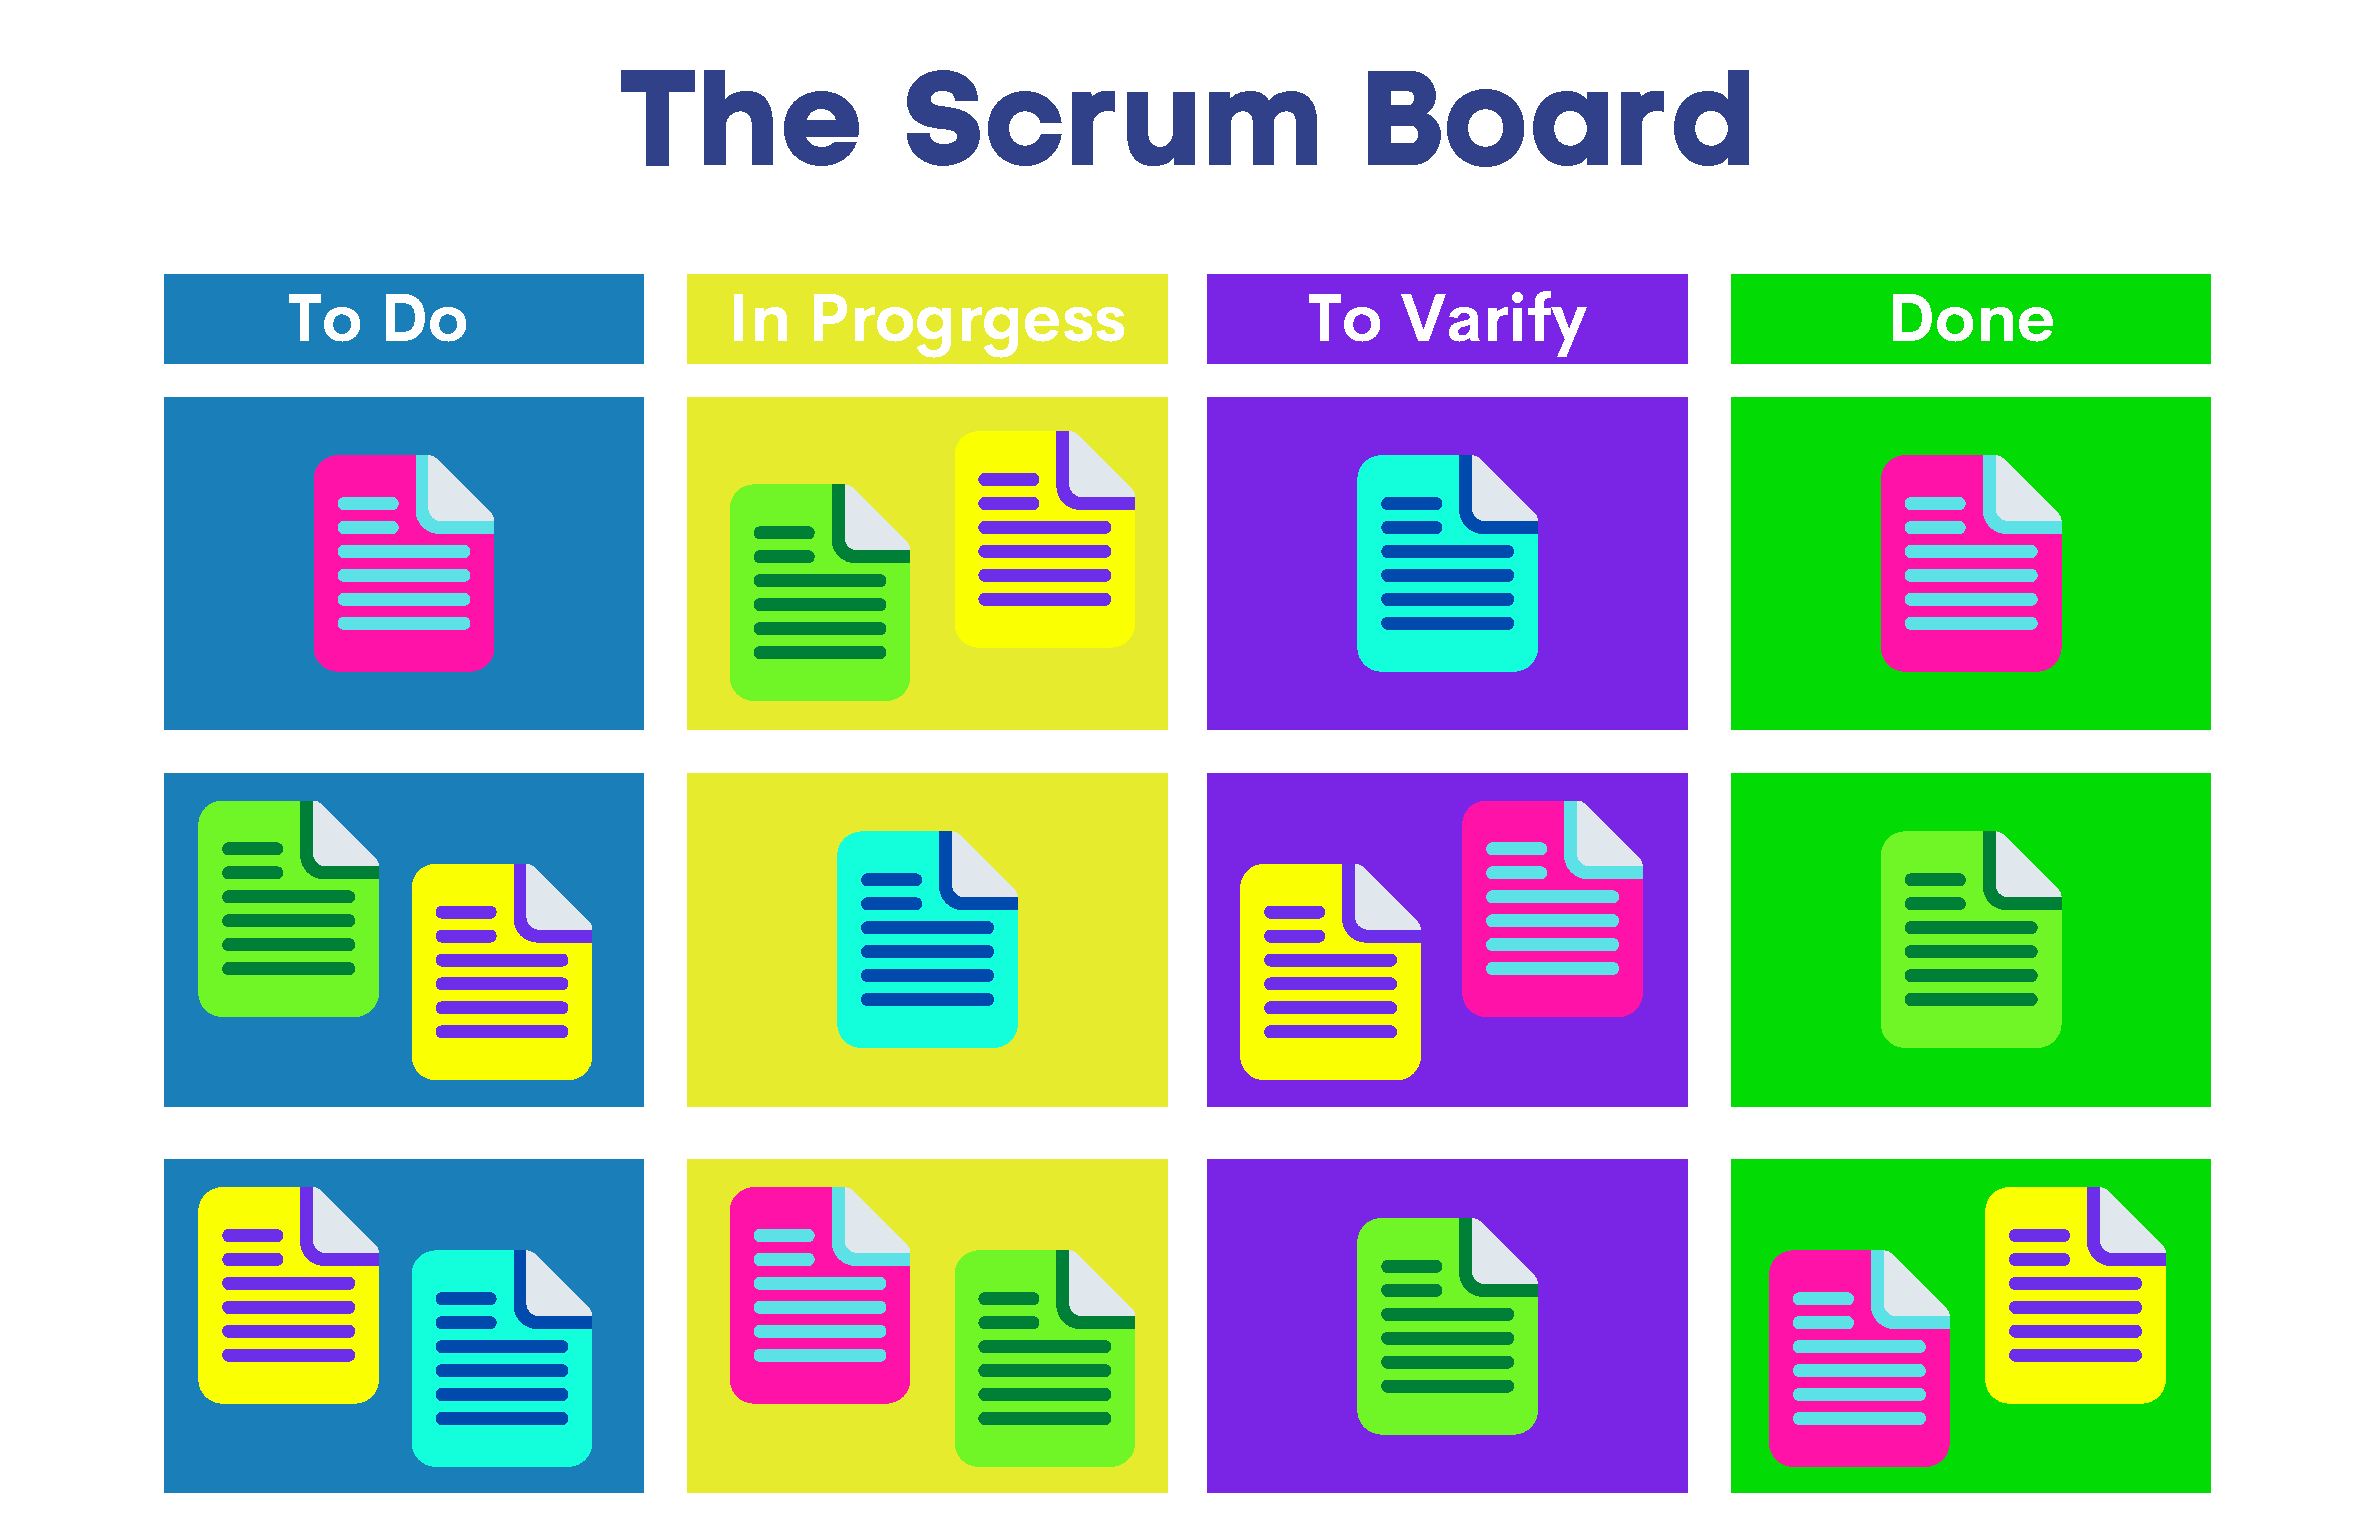
\includegraphics[width=1\textwidth]{images/scrum_board}
    \caption{Project Management Agile Scrum Board Template}
    \label{fig:scrum_board}
\end{figure}


To fulfill the desire of a scrum board we use ``Trello" which is an online tool to help creating Scrum board. Below is an example of a Scrum board in Trello of our project work.

\begin{figure}[H]
    \centering
    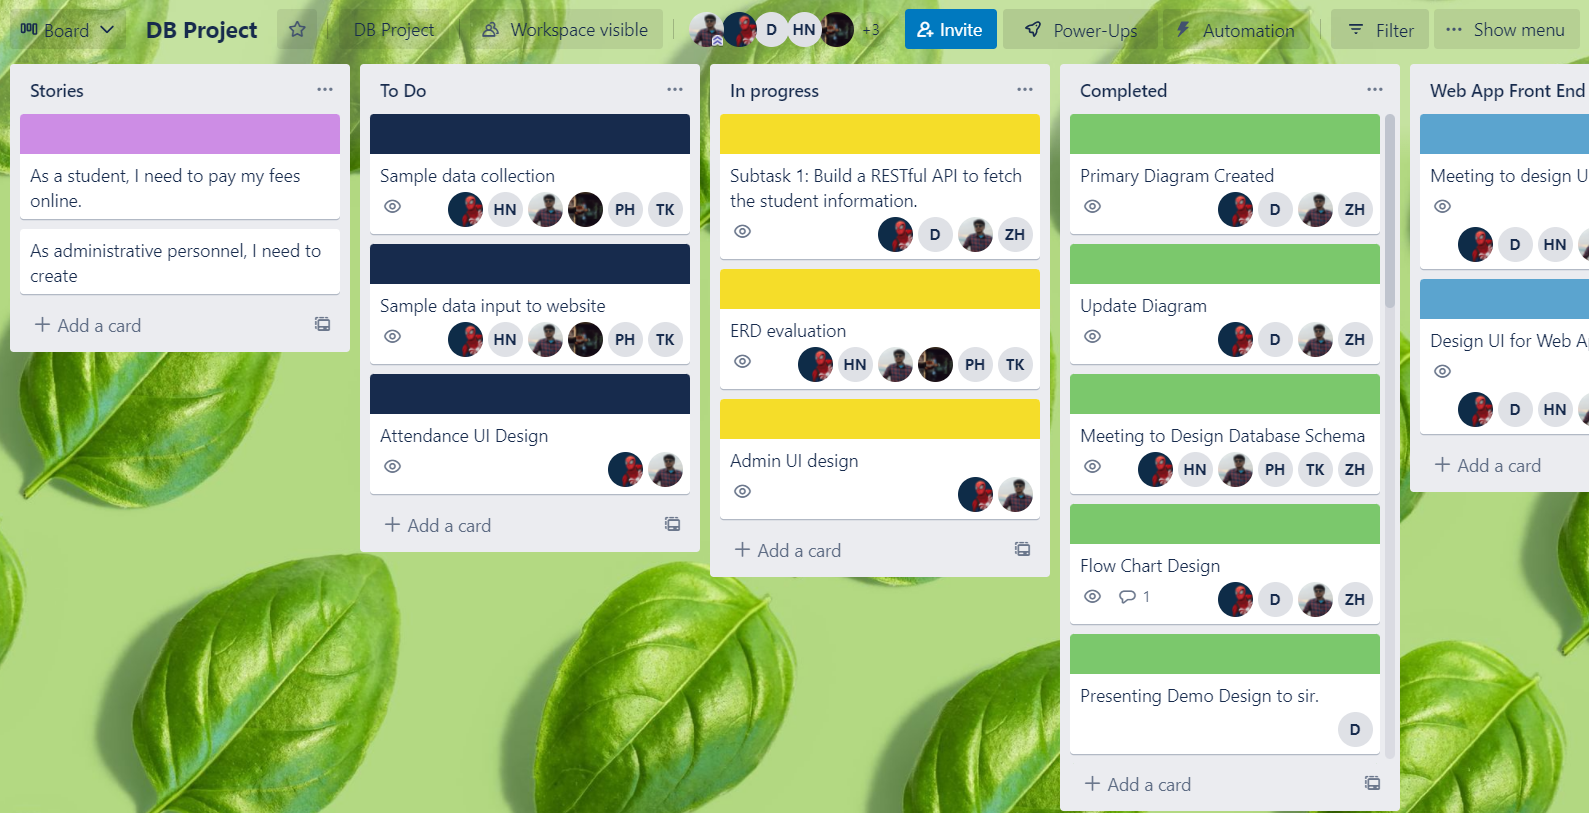
\includegraphics[width=1\textwidth]{images/trello}
    \caption{Example of Trello of CU-OPAS}
    \label{fig:trello}
\end{figure}

We can easily maintain our scrum board using Trello. After completing a task on a specific field we can easily move it to another field using drag and drop property. This makes our work more easier. Aslo, a important property of Trello is that, we can assign each and every task with a deadline to a specific member of our scrum team. According to deadline, our members complete the task assigned to him.


%Using the cards, you may describe the specifics of the tasks, such as who will be assigned to the job, what will be done, when it will be completed, and so on. Additionally, we utilized these cards to keep track of our meeting schedule and information, as well as any future revisions. In addition to the ``To Do" lists, the task board also had columns for ``Work In Progress," ``Testing," and ``Work Done," as well as a column for "Testing." A typical task board is shown in the diagram below.\\%

\item \textbf{Testing and Product Demonstration}\\

Generally, after each iteration, the development team creates a new version of a software product with increased value. Stack-holders and customers which includes students, teachers, and other relevant authorities reviews our system in this step. They provide their valuable comments. If every thing is positive, then the respective sprint is successful. Otherwise, we make some modification depending on the results of the study.

\item \textbf{Retrospective and the next sprint planning}\\

After completing all the previous steps, it is necessary to examine what is gone well and what might be improved for the following level. We speaks about the lessons gained and the hazards of any specific challenges or problems that come up throughout the course of the project. We discusses our next sprint, which will consist of future development. An important feature is that at this stage it is the processes of work and interaction that are discussed in order to improve the work of the Scrum team as a whole. We finally conclude what went well during the working process and what can be done better during future iteration. Then concentrate on the next sprint planning.

\end{enumerate}

%Each and every member of our team has made an equal contribution to the project, from the beginning of the planning phase to the completion of the system's final implementation. We attempted to create a better system than the present one, and after hundreds of proposals were discussed and rejected by all of us, we were eventually successful. In order to accomplish this project, we attempted to make the best possible use of existing technology. During the course of the project, we discovered a great deal of new information while being stuck on challenges we had never encountered before. Projects might be conducted carelessly if adequate project management principles are not followed, putting them at a much greater risk of failure, delay, and going over budget. Knowing the foundations of project management increased our chances of effectively completing a project. According to this procedure we complete all of the steps of SDLC and our project completes.%

\clearpage